\chapter{膨胀的牛顿宇宙}

\lectureoverview{现代宇宙学始于把宇宙本身当作一个物理系统来处理。从大尺度各向同性和均匀性出发，我们引入共动网格，并将其运动编码在单个标度因子\(a(t)\)中。牛顿壳层定理随后把引力多体问题化为关于\(a(t)\)的方程。能量守恒区分了再坍缩、临界和永远膨胀的宇宙，而临界的物质主导情形给出第一个弗里德曼方程以及规律\(a(t)\propto t^{2/3}\)。}

\section{宇宙学何时成为物理学}

宇宙学作为一门学科古已有之，但定量宇宙学还很年轻。就目前的目的而言，没有必要从希腊人开始。有用的历史起点是哈勃在二十世纪第二个四分之一世纪对宇宙膨胀的发现，以及后来把大约三开尔的微波背景确认为炽热早期宇宙的遗迹。

在测量变得精确之前，天文学的大部分内容必然类似于自然史。人们发现一颗不寻常的恒星，把某个特殊星系分类，测量能够测量的东西，并汇编一份天体目录。那些天体当然是物理系统：它们携带角动量，含有化学元素，并服从力学。决定性的变化是把\emph{整个宇宙}当作一个物理系统，由精确到足以与观测相对照的方程支配。

这就是本书的主题。我们不会仅仅罗列宇宙的内容物；我们要追问它的变量、它的运动和它的动力学定律。方程不是事后添加的装饰。它们是使宇宙成为一个物理学问题的手段。

从历史上看，膨胀宇宙是用广义相对论的语言来理解的。然而从逻辑上看，第一个论证的很大一部分是牛顿式的。一位猜对了正确大尺度运动的十七世纪物理学家本可以推导出一个相当好的模型。从牛顿开始，并不是要取代相对论，而是要揭示后来被相对论以几何方式重新组织起来的力学。

\section{各向同性、均匀性与宇宙学原理}

第一步是观测性的。在足够大的尺度上，宇宙近似是\emph{各向同性}的：在对天空的若干区域取平均并越过银河系的前景之后，它在每个方向上看起来都大致相同。这并不是说它精确均匀。直接看一颗近处的恒星与看一片空区域是不同的，而物质分布包含真实的结构。各向同性是一个经过平均的大尺度陈述。

均匀性是一个不同的陈述。它说的是，经过平均的宇宙从一个地方到另一个地方都相同。一位身处许多星系之外的观测者，在作同样的大尺度平均之后，应当看到与我们所见大致相同类型的宇宙。

作为第一级近似，一个星系可以简单地当作一个质点来处理。可见宇宙中大约有
\begin{equation}
N_{\rm gal}\sim 10^{11}
\end{equation}
个星系，每个星系有大约\(10^{11}\)颗恒星。这给出大约\(10^{22}\)颗恒星。如果刻意用每颗恒星十颗行星作为粗略的数量级估计，就得到\(10^{23}\)颗行星，有趣的是这接近一摩尔的行星。这个数值估计并不属于动力学的一部分，但它确定了正在被理想化的系统的尺度。

\begin{classroomqa}
\classquestion{在可观测宇宙内，按数量级说有多少个星系？}
\lecturerresponse{大约一千亿个，即\(10^{11}\)。以每个星系大约\(10^{11}\)颗恒星计，这意味着可见宇宙中大约有\(10^{22}\)颗恒星。这些是有用的尺度估计，值得记住，尽管下面的计算把每个星系替换为一个质点。\lecturetimestamp{00:06:08--00:07:05}}
\end{classroomqa}

为什么我们周围的各向同性应当暗示均匀性？想象一个各向同性但\emph{不}均匀的分布。它的密度就必须随离我们的距离而变化，同时保持与方向无关：实际上，它会围绕我们的位置形成一种同心壳层的图样。一位偏离共同中心的观测者就不会再看到各向同性。因此有两种可能：
\begin{enumerate}
\item 我们占据着一个特殊的中心，宇宙是围绕它安排好的；或者
\item 大尺度分布近似均匀，因此没有任何被占据的点是特殊的。
\end{enumerate}
第二种可能更经济。各向同性，加上拒绝赋予我们自己一个享有特权的宇宙位置，导致均匀性。

\begin{classroomqa}
\classquestion{各向同性但不均匀的分布可能采取什么形式？}
\lecturerresponse{它的变化可以只依赖于离我们的距离，从而产生以我们的位置为中心的壳层状图样。把观测者移离那个中心，图样就不再是各向同性的。除非我们的位置特殊，各向同性因此指向均匀性。\lecturetimestamp{00:07:06--00:08:54}}
\end{classroomqa}

这一组合假设被称为\emph{宇宙学原理}：在足够大的尺度上，宇宙在空间上是均匀且各向同性的。称之为原理并不能证明它。历史上，宇宙学家在观测强有力地证成它之前就采纳了这一假设。它的地位来自经验上的成功。

均匀性也并非严格成立。星系会形成星系团和超星系团，而且长期以来一直有关于延伸到可见天空极大一部分的结构的讨论。恰当的说法是，当平均区域足够大时---在本入门讨论中约为数亿到大约十亿光年量级，涨落会被平均掉。这一尺度可以通过观测加以修正；方法是不断粗粒化，直到局部结构不再主导描述。

\begin{classroomqa}
\audiencequestion{宇宙微波背景的均匀性是否为宇宙学原理提供了证据？}
\lecturerresponse{是的。宇宙学原理是在尚无强有力的观测依据时被提出的，但微波背景后来表明，原初宇宙极其平滑。星系和星系团由对这一平滑状态的微小偏离生长而来；它们并不抹去支持它的大尺度证据。\lecturetimestamp{00:10:53--00:11:43}}
\end{classroomqa}

\section{随星系一起运动的网格}

一旦选定了观测近似，我们就必须选择变量。对于“表述一个物理问题的第一步是什么？”这个问题，一种课堂答案是知道变量；传统的答案是削尖铅笔。在这里，重要的变量通过恰当地选择坐标而找到。

想象一个带有标记\(x,y,z\)的三维网格。这些标记不必是用米测量的距离。它们是坐标数。选择网格，使得在小的本动运动被平均掉之后，每个星系都停留在固定的网格点上。星系于是就是\emph{共动的}。

如果星系随机运动，这样的选择将毫无用处。观测反而揭示出一种相干的大尺度运动。相邻的网格单元可以膨胀或收缩，但同样的膨胀或收缩处处发生。因此，所有物理距离都可以写成一个共同的时间相关尺度乘以固定的坐标间隔。

对于两个星系\(A\)和\(B\)，
\begin{equation}
\begin{aligned}
d_{AB}(t)&=a(t)\,\Delta\chi_{AB},\\
\Delta\chi_{AB}
&=\sqrt{(x_A-x_B)^2+(y_A-y_B)^2+(z_A-z_B)^2}.
\end{aligned}
\label{eq:c01-physical-distance}
\end{equation}
如果它们只在\(x\)坐标上不同，这简化为
\begin{equation}
d_{AB}(t)=a(t)\,\Delta x_{AB}.
\end{equation}
函数\(a(t)\)是\emph{标度因子}。它的绝对归一化是约定性的：把所有共动坐标乘以一个常数并把\(a\)除以同一个常数，不改变任何物理距离。诸如\(a(t_2)/a(t_1)\)这样的比值，以及除以\(a\)的导数，携带着物理信息。

对式~\eqref{eq:c01-physical-distance}求导。共动间隔是固定的，所以
\begin{equation}
v_{AB}=\dot a\sqrt{(\Delta x)^2+(\Delta y)^2+(\Delta z)^2}.
\end{equation}
除以物理距离得到
\begin{equation}
\frac{v_{AB}}{d_{AB}}=\frac{\dot a}{a}\equiv H(t),
\label{eq:c01-hubble-parameter}
\end{equation}
或
\begin{equation}
\boxed{v_{AB}=H(t)d_{AB}.}
\label{eq:c01-hubble-law}
\end{equation}
这就是理想均匀流中的哈勃定律。

“哈勃常数”这个名字可能引起误解。在某一宇宙时刻，\(H\)的同一个值适用于均匀模型中的每一个地点，但\(H(t)\)一般随时间变化。空间上的普适性并不是时间上的恒常性。

\begin{classroomqa}
\audiencequestion{通过把每个距离写成一个共同的\(a(t)\)乘以固定的坐标间隔，我们是否已经假定了哈勃定律？}
\lecturerresponse{这一拟设当然是由哈勃的观测所激发的；若没有相干退行的证据，就不会猜到它。它的价值在于组织那些证据。不必给每个星系指定一个独立的速度，而是描述一个单一的膨胀网格。一旦采纳了这一描述，比例关系\(v=Hd\)便通过求导得出。\lecturetimestamp{00:24:20--00:25:33}}
\end{classroomqa}

同一种运动容许两种文字描述。人们可以说星系穿过空间彼此远离，也可以说星系停留在固定的共动位置上，而网格---因而它们之间的物理空间---在膨胀。在这个阶段，它们是同一套数学的两种坐标描述。广义相对论将使膨胀空间的语言特别自然，但没有任何观测能区分在每一时刻都给出相同物理间隔的两种描述。

\section{共动元胞中的质量记账}

在引入引力之前，先追踪质量。考虑一个小的坐标元胞，其坐标体积为
\begin{equation}
\Delta V_{\rm com}=\Delta x\,\Delta y\,\Delta z.
\end{equation}
它仍必须足够大，以包含许多星系，从而可以平均掉局部涨落。令\(\nu\)表示每单位共动坐标体积的质量。该元胞中的质量为
\begin{equation}
\Delta M=\nu\,\Delta x\,\Delta y\,\Delta z.
\label{eq:c01-comoving-mass}
\end{equation}
因为该元胞随物质一起运动，在理想流动中没有星系穿过其边界，所以\(\Delta M\)是常量。

每条物理边都比其坐标边长一个因子\(a(t)\)。因此物理体积为
\begin{equation}
\Delta V_{\rm phys}=a^3(t)\,\Delta x\,\Delta y\,\Delta z.
\end{equation}
物理质量密度为
\begin{equation}
\boxed{\rho(t)=\frac{\Delta M}{\Delta V_{\rm phys}}=\frac{\nu}{a^3(t)}.}
\label{eq:c01-density-dilution}
\end{equation}
膨胀将无压物质稀释为\(a^{-3}\)；收缩则按同样的规律将其浓缩。

到此为止，尚未假设任何动力学内容。我们使用了欧几里得几何、一个运动学假设，以及共动元胞中的质量守恒。现在引力登场了。

\section{现在牛顿登场}

一个诱人但不正确的图景认为，无限均匀的物质分布应当保持静止，因为一侧的拉力被另一侧的拉力抵消了。其缺陷在于，这种非正式的抵消并不能为相对加速度提供一个自洽的方程。牛顿的球壳定理给出了力的正确组织方式。

任选一个星系作为原点\(O\)，并考虑一个位于固定共动半径处的星系\(A\)
\begin{equation}
R=\sqrt{x^2+y^2+z^2}.
\end{equation}
它的物理半径、径向速度和径向加速度为
\begin{equation}
d=aR,
\qquad
\dot d=\dot a R,
\qquad
\ddot d=\ddot a R.
\label{eq:c01-radial-kinematics}
\end{equation}

\begin{figure}[ht]
\centering
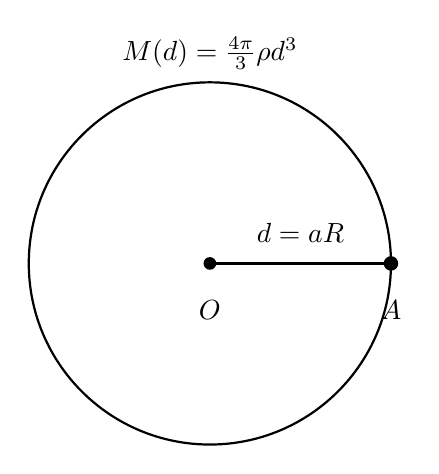
\begin{tikzpicture}[scale=1.15]
\draw[thick] (0,0) circle (2);
\fill (0,0) circle (0.07);
\fill (2,0) circle (0.08);
\draw[thick] (0,0) -- (2,0);
\draw (1,0.12) node[above] {\(d=aR\)};
\draw (0,-0.3) node[below] {\(O\)};
\draw (2,-0.3) node[below] {\(A\)};
\draw (0,2.32) node {\(M(d)=\frac{4\pi}{3}\rho d^3\)};
\end{tikzpicture}
\caption{牛顿式约化。对于星系\(A\)的加速度，外部球壳的贡献相互抵消，而半径\(d\)以内的质量表现得如同集中在\(O\)处。}
\label{fig:c01-newton-sphere}
\end{figure}

对于球对称的质量分布，来自通过\(A\)的球面之外物质的净力为零。球面内的物质表现得如同集中在中心。所包围的质量为
\begin{equation}
M(d)=\frac{4\pi}{3}\rho d^3.
\label{eq:c01-enclosed-mass}
\end{equation}
牛顿的平方反比定律于是给出\(A\)的加速度：
\begin{equation}
\ddot d=-\frac{GM(d)}{d^2}.
\end{equation}
利用方程~\eqref{eq:c01-radial-kinematics}，
\begin{align}
\ddot a R
&=-\frac{G}{d^2}\left(\frac{4\pi}{3}\rho d^3\right) \\
&=-\frac{4\pi G}{3}\rho d \\
&=-\frac{4\pi G}{3}\rho aR.
\end{align}
共动半径被消去，留下
\begin{equation}
\boxed{\frac{\ddot a}{a}=-\frac{4\pi G}{3}\rho.}
\label{eq:c01-acceleration}
\end{equation}
这种消去就是自洽性检验。每一个共动星系，无论其\(R\)如何，都遵循同一个关于同一标度因子的方程。

代入方程~\eqref{eq:c01-density-dilution}得到两种等价形式中的任一种
\begin{equation}
\frac{\ddot a}{a}=-\frac{4\pi G\nu}{3a^3},
\qquad
\ddot a=-\frac{4\pi G\nu}{3a^2}.
\label{eq:c01-acceleration-nu}
\end{equation}
第一种形式展示的是分数加速度；第二种形式将\(\ddot a\)分离出来。把\(a\)保留在左边是一种约定，而不是物理上的改变。

\begin{classroomqa}
\audiencequestion{原点是任意选取的，然而计算中的每一个力都指向它。为什么选择不同的原点会给出同一个宇宙？}
\lecturerresponse{该方程涉及的是相对运动。围绕任何其他星系重复计算都会得到同一个方程，因为均匀性使得所包围的质量只依赖于物理半径。如果变换到一个附着于另一个星系的加速参考系，同时保留相对于第一个原点表述的力，那么相应的惯性力也必须被纳入。选择一个中心静止参考系只是避免了额外的记账工作。不变的结果是方程~\eqref{eq:c01-acceleration}，而不是某个特殊的中心。\lecturetimestamp{00:43:56--00:46:58}}
\end{classroomqa}

\begin{classroomqa}
\audiencequestion{如果共动质量密度\(\nu\)逐处变化，这一结果还能成立吗？}
\lecturerresponse{不能以这种单函数形式成立。干净的消去依赖于\(M\propto d^3\)在各处具有相同的比例关系。如果\(\nu\)在平均尺度上变化显著，不同区域将需要不同的局部动力学，而单一的均匀标度因子将不再能描述它们。均匀性在做着本质性的工作。\lecturetimestamp{00:47:05--00:47:51}}
\end{classroomqa}

\begin{classroomqa}
\audiencequestion{为什么写成\(\ddot a/a\)，而不是把因子\(a\)移到右边？}
\lecturerresponse{两种形式都正确。宇宙学惯例上写成分数加速度\(\ddot a/a\)，部分原因是它可以与分数膨胀率\(H=\dot a/a\)直接比较。两边乘以\(a\)得到完全相同的微分方程。\lecturetimestamp{00:50:36--00:51:29}}
\end{classroomqa}

方程~\eqref{eq:c01-acceleration}立即排除了一个充满普通物质的静态均匀牛顿宇宙。静态标度因子会有\(\ddot a=0\)，而正密度使右边为负。这\emph{尚未}告诉我们宇宙是在膨胀还是在收缩。它只告诉我们加速度的符号。

\section{负加速度不是收缩}

速度与加速度之间的区别是初等的，但却是决定性的。一辆在高速公路上向前行驶的法拉利可以具有正速度，同时以负加速度刹车。同样，一个宇宙可以有
\begin{equation}
\dot a>0,
\qquad
\ddot a<0:
\end{equation}
它在膨胀，但膨胀正在减慢。

要判断运动最终是否会反向，可以把宇宙学问题与一个在 Earth 引力场中沿径向运动的检验粒子作比较。现在令 \(x\) 表示该粒子到中心质量 \(M\) 的物理距离；它与先前的共动坐标无关。Newton 方程为
\begin{equation}
\ddot x=-\frac{GM}{x^2}.
\label{eq:c01-particle-force}
\end{equation}
加速度始终指向内部。一个被向外抛出的粒子仍可能长时间地、甚至永远地继续向外运动。一个已经在向内运动的粒子会获得越来越负的速度。仅凭力定律并不能决定发生哪种运动；初始条件才能决定。

\begin{classroomqa}
\audiencequestion{\(\ddot a<0\) 是否意味着宇宙正在收缩？}
\lecturerresponse{不。收缩意味着 \(\dot a<0\)。负的 \(\ddot a\) 只意味着 \(\dot a\) 随时间减小。如果 \(\dot a\) 一开始为正，引力会使膨胀减慢；它是否会达到零取决于初始膨胀速率，正如一个向外运动的抛射体的命运取决于它低于还是高于逃逸速度。\lecturetimestamp{00:51:30--00:56:18}}
\end{classroomqa}

\begin{figure}[ht]
\centering
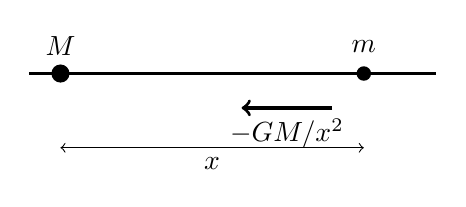
\begin{tikzpicture}[scale=1.15]
\fill (0,0) circle (0.1);
\draw (0,0.3) node {\(M\)};
\draw[thick] (-0.35,0) -- (4.15,0);
\fill (3.35,0) circle (0.08);
\draw (3.35,0.3) node {\(m\)};
\draw[->,very thick] (3.0,-0.38) -- (2.0,-0.38)
  node[midway,below] {\(-GM/x^2\)};
\draw[<->] (0,-0.82) -- (3.35,-0.82)
  node[midway,below] {\(x\)};
\end{tikzpicture}
\caption{用来把加速度的符号与运动的方向和命运区分开的径向单粒子问题。}
\label{fig:c01-particle-sketch}
\end{figure}

能量使这些可能性变得一目了然。守恒的机械能为
\begin{equation}
E=\frac12 m\dot x^{\,2}-\frac{GMm}{x}.
\label{eq:c01-particle-energy}
\end{equation}
势能与 \(1/x\) 成正比，而不是与 \(1/x^2\) 成正比；对 \(-GMm/x\) 求导会产生平方反比力。

\begin{figure}[ht]
\centering
\includegraphics[width=0.82\textwidth]{lecture_01_figure_02.png}
\caption{能量论证开始时的板书：一个运动的检验质量及其动能项，就在引力势能被恢复之前。}
\lectureframe{00:58:57}
\end{figure}

如果 \(E<0\)，一个向外运动的粒子无法到达无穷远，在那里它的势能趋于零而动能非负。它必须在有限的 \(x\) 处停下并返回。如果 \(E>0\)，它无法停下，因为在转折点处动能会变为零，而剩余的势能会是负的，这与正的 \(E\) 守恒相矛盾。边界为
\begin{equation}
E=0,
\end{equation}
它定义了逃逸速度：
\begin{equation}
\frac12 m v_{\rm esc}^2-\frac{GMm}{x}=0,
\qquad
\boxed{v_{\rm esc}^2=\frac{2GM}{x}.}
\label{eq:c01-escape-velocity}
\end{equation}

\begin{figure}[ht]
\centering
\includegraphics[width=0.88\textwidth]{lecture_01_figure_03.png}
\caption{零能量边界正在黑板上成形。先前的宇宙学加速度方程仍被框在左侧，而径向逃逸问题在右侧展开。}
\lectureframe{01:01:37}
\end{figure}

恰好在逃逸速度时，粒子会无限地减慢。只有当 \(x\to\infty\) 时，它的速率才趋于零；它永远不会到达一个有限的转折点。这个边缘情形将是最简单的宇宙学模型。

\section{宇宙学能量方程}

回到一个位于固定共动半径 \(R\) 处的星系。根据球壳定理，它的径向运动与一个在点质量外部运动的粒子相同，该点质量等于其共动球所包围的质量。

\begin{figure}[ht]
\centering
\includegraphics[width=0.82\textwidth]{lecture_01_figure_04.png}
\caption{当单粒子能量论证被转回宇宙学时所用的平方反比力和径向粒子示意图。}
\lectureframe{01:04:14}
\end{figure}

被包围的质量不会随着物理球的膨胀而增加。该球是共动的，因此它始终包含相同的星系：
\begin{align}
M
&=\frac{4\pi}{3}\rho(aR)^3 \\
&=\frac{4\pi}{3}\frac{\nu}{a^3}a^3R^3 \\
&=\frac{4\pi}{3}\nu R^3.
\label{eq:c01-fixed-enclosed-mass}
\end{align}
第一个表达式只有在把密度稀释包括进来之前才显得依赖于时间。\(a^3\) 的因子会相消。

\begin{classroomqa}
\audiencequestion{随着球的膨胀，它包围的质量会增加吗？}
\lecturerresponse{不会。它的物理半径在增长，但它的共动边界随星系一起运动。在理想均匀流中，没有物质穿过该边界，而方程~\eqref{eq:c01-fixed-enclosed-mass}明确显示了这种相消。\lecturetimestamp{01:04:37--01:05:20}}
\end{classroomqa}

该星系的物理速度为 \(\dot d=\dot a R\)，它到所选原点的距离为 \(d=aR\)。因此它守恒的 Newton 能量为
\begin{equation}
\boxed{
E=\frac12 m\dot a^{\,2}R^2-\frac{GMm}{aR}.
}
\label{eq:c01-cosmological-energy}
\end{equation}

\begin{figure}[ht]
\centering
\includegraphics[width=0.82\textwidth]{lecture_01_figure_05.png}
\caption{黑板上的宇宙学动能项和势能项。方程~\eqref{eq:c01-cosmological-energy}中完整的分母 \(aR\) 来自物理半径以及相应的推导。}
\lectureframe{01:06:12}
\end{figure}

三种粒子能量情形变为三种宇宙学情形：
\begin{description}[style=nextline]
\item[\(E<0\)：]初始膨胀低于逃逸速度；\(a(t)\)达到最大值，宇宙重新坍缩。
\item[\(E=0\)：]宇宙恰好处于临界状态；膨胀永远减慢，仅渐近地趋近于零速度。
\item[\(E>0\)：]初始膨胀高于逃逸速度；在牛顿模型中，宇宙永远膨胀，具有非零的渐近退行速度。
\end{description}

我们从边界情形\(E=0\)开始。将方程~\eqref{eq:c01-cosmological-energy}设为零，消去\(m\)，并除以\(a^2R^2/2\)，得到
\begin{align}
\frac12\dot a^{\,2}R^2&=\frac{GM}{aR}, \\
\left(\frac{\dot a}{a}\right)^2&=\frac{2GM}{a^3R^3}.
\label{eq:c01-energy-intermediate}
\end{align}
由于
\begin{equation}
\rho=\frac{M}{(4\pi/3)a^3R^3},
\end{equation}
方程~\eqref{eq:c01-energy-intermediate}变为
\begin{equation}
\boxed{
H^2=\left(\frac{\dot a}{a}\right)^2=\frac{8\pi G}{3}\rho.
}
\label{eq:c01-first-friedmann}
\end{equation}
这就是空间平坦、仅含物质、宇宙学常数为零的宇宙的第一弗里德曼方程，此处由牛顿能量守恒得到。

\begin{classroomqa}
\classquestion{以恰好等于逃逸速度发射的粒子会发生什么？}
\lecturerresponse{它会减慢，但永远不会反向。其速率仅在无穷远处才趋近于零。零能量宇宙的行为方式相同：\(H\)减小，但\(\dot a\)保持为正，不会发生有限时间的回转。\lecturetimestamp{01:10:45--01:12:10}}
\end{classroomqa}

因子\(4\pi/3\)和\(8\pi G/3\)并非随意的装饰。\(4\pi/3\)是球的体积，而因子二来自动能。在广义相对论中，同一个\(8\pi G\)出现在爱因斯坦场方程中，其时间-时间分量导致相对论性的弗里德曼方程。这种一致并非偶然，但目前的推导尚未包括压强、作为几何的空间曲率或宇宙学常数。

\section{临界物质主导解}

在方程~\eqref{eq:c01-first-friedmann}中使用密度定律\(\rho=\nu/a^3\)：
\begin{equation}
\left(\frac{\dot a}{a}\right)^2=\frac{8\pi G\nu}{3a^3}.
\label{eq:c01-matter-friedmann}
\end{equation}
常数\(\nu\)依赖于共动坐标的任意归一化。为了揭示时间依赖性，定义
\begin{equation}
K\equiv\frac{8\pi G\nu}{3}>0.
\end{equation}
于是
\begin{equation}
\dot a^{\,2}=\frac{K}{a}.
\label{eq:c01-normalized-friedmann}
\end{equation}

\begin{figure}[ht]
\centering
\includegraphics[width=0.76\textwidth]{lecture_01_figure_06.png}
\caption{黑板上的物质主导弗里德曼标度关系，先写出其常数，然后揭示标度因子的本质性反比幂。}
\lectureframe{01:14:44}
\end{figure}

方程~\eqref{eq:c01-normalized-friedmann}的右侧在每个有限正\(a\)处均为正。回转将要求\(\dot a=0\)，因此临界宇宙永远不会回转。其膨胀变得越来越疲惫，但永远不会疲惫到停止。

现在求解该方程。可以直接分离变量，
\begin{equation}
a^{1/2}\,da=\sqrt{K}\,dt,
\end{equation}
或者按照讲座尝试幂律，
\begin{equation}
a(t)=Ct^p.
\label{eq:c01-power-trial}
\end{equation}
于是
\begin{equation}
\frac{\dot a}{a}=\frac{p}{t},
\qquad
\frac{K}{a^3}=\frac{K}{C^3t^{3p}}.
\end{equation}
代入方程~\eqref{eq:c01-matter-friedmann}得到
\begin{equation}
\frac{p^2}{t^2}=\frac{K}{C^3t^{3p}}.
\end{equation}
匹配幂次和系数得到
\begin{equation}
3p=2,
\qquad
C^3=\frac{K}{p^2}=\frac{9K}{4}.
\end{equation}
因此
\begin{equation}
\boxed{
a(t)=\left(\frac{3\sqrt K}{2}t\right)^{2/3}\propto t^{2/3}.
}
\label{eq:c01-two-thirds}
\end{equation}
时间的可加原点已被选定，使得在\(t=0\)时\(a=0\)。更一般地，可以将\(t\)替换为\(t-t_0\)。

标度因子永远增长，而
\begin{equation}
\dot a\propto t^{-1/3}\longrightarrow0,
\qquad
H=\frac{2}{3t}\longrightarrow0.
\label{eq:c01-asymptotic-slope}
\end{equation}
其图像始终递增且始终向下凹。它不趋近于任何水平线，因为\(a(t)\)本身无界，但其斜率趋于零。

\begin{classroomqa}
\audiencequestion{\(t^{2/3}\)是否仅仅因为该试探形式恰好奏效才被找到？另一种试探能否给出另一个零能量解？}
\lecturerresponse{该试探确定的是解，而不仅仅是某一种可能性。一阶膨胀分支方程\(\dot a=\sqrt{K/a}\)积分后唯一地给出\(a\propto(t-t_0)^{2/3}\)，至多相差归一化和时间原点的选择。不同的总能量给出不同的微分方程，因而给出不同的宇宙学历史。\lecturetimestamp{01:27:07--01:27:43}}
\end{classroomqa}

\begin{classroomqa}
\audiencequestion{临界曲线最终会变为水平吗？}
\lecturerresponse{其斜率趋于零：\(\dot a\propto t^{-1/3}\)。然而它在每个有限时刻均为正，因此标度因子继续无界增长。宇宙渐近地趋近于静止，但永远不会达到静止。\lecturetimestamp{01:27:48--01:28:57}}
\end{classroomqa}

这个简单的结果在历史上引人注目。牛顿拥有推导所需的力学和球壳定理，并且他考虑过关于无限引力宇宙的问题，但他没有提出膨胀模型。课堂讨论表明，关于宇宙历史的哲学和神学承诺可能影响了他认为哪些问题是自然的。这一历史推测不属于推导的一部分；数学上的要点仅仅是所需的牛顿工具当时已经存在。

\begin{classroomqa}
\audiencequestion{这个牛顿式构造是否假设宇宙无限？}
\lecturerresponse{它假设的是欧几里得、空间平坦的牛顿空间。在通常的牛顿模型中，该空间无限延伸，因此即便共动星系之间的距离随时间变化，该模型在空间上仍是无限的。弯曲的有限空间几何属于相对论处理的范围。\lecturetimestamp{01:22:12--01:22:55}}
\end{classroomqa}

\section{超越零能量模型}

零能量情形是一种有意的简化，而不是唯一的牛顿宇宙。保留方程~\eqref{eq:c01-cosmological-energy}中的\(E\neq0\)，得到
\begin{equation}
\left(\frac{\dot a}{a}\right)^2
=\frac{8\pi G}{3}\rho+\frac{2E}{mR^2a^2}.
\label{eq:c01-nonzero-energy}
\end{equation}
均匀性要求组合\(2E/(mR^2)\)对每一个代表性共动球都相同。将其写为常数\(C_E\)，
\begin{equation}
H^2=\frac{8\pi G}{3}\rho+\frac{C_E}{a^2}.
\end{equation}
正的\(C_E\)对应于能量高于逃逸；负的\(C_E\)允许发生回转。在相对论记号中，这一能量项通过空间曲率被重新解释，这一联系留待后续处理。

在物质主导期间，这三种仅含物质的历史都具有负加速度：
\begin{equation}
\ddot a=-\frac{4\pi G}{3}\rho a<0.
\end{equation}
再坍缩曲线上升，达到\(\dot a=0\)，然后下降。临界曲线\(t^{2/3}\)永远上升，斜率趋于零。正能量曲线也永远上升，并趋近线性增长。课上曾对这些情形作过临时板书草图，后来作了更正；稳定的结论是它们共同具有凹向下的行为，而不是第一幅草图的每一个细节。

观测到的宇宙还有更多表现。其早期物质主导的膨胀可以用一条减速曲线很好地近似，但在晚期，该曲线向上弯曲：
\begin{equation}
\ddot a>0.
\end{equation}
普通无压物质无法在方程~\eqref{eq:c01-acceleration}中产生这种符号。因此需要一个额外项。在最简单的现代模型中，它是宇宙学常数；更一般地，它被称为暗能量。本章有意省略它，以便首先清晰地理解牛顿物质动力学。

\begin{classroomqa}
\audiencequestion{弗里德曼方程中的\(8\pi G\)是否与爱因斯坦场方程中出现的因子相同，我们是否包含了宇宙学常数？}
\lecturerresponse{同一个引力归一化因子也出现在广义相对论中，而时间-时间场方程重现了相对论弗里德曼方程。这里的模型不包含宇宙学常数。它是一个物质主导的宇宙；缺失的宇宙学常数项正是那种能够解释晚期加速的项。\lecturetimestamp{01:30:15--01:31:06}}
\end{classroomqa}

\section{平均流动与局部偏离}

均匀膨胀是一种粗粒化描述。它并不是说每个物体都会远离每一个邻近物体。受引力束缚或以其他方式束缚的系统可以与哈勃流解耦。例如，银河系和仙女座星系彼此接近，而不是遵循大尺度退行定律。

单个星系的速度偏离哈勃流的部分称为其\emph{本动速度}。这个术语是技术性的，并不是对星系的评判。当人们对更大的距离和更大的体积取平均时，哈勃定律会成为更好的近似。在束缚星系、星系团或局部过密区域的尺度上，局部力可以主导背景膨胀。

\begin{classroomqa}
\audiencequestion{即使宇宙整体膨胀，某些区域能否收缩？}
\lecturerresponse{当然可以。束缚系统和足够致密的涨落不必遵循平均膨胀。银河系--仙女座星系系统就是一个熟悉的例子。宇宙学计算是在足够大的体积上取平均，使得这些本动运动和局部密度涨落不占主导；由此得到的\(a(t)\)描述的是背景，而不是每一对物体。\lecturetimestamp{01:31:00--01:34:13}}
\end{classroomqa}

类比是普通气体。说房间里的空气是均匀的，并不否认分子涨落或密度的局部变化。它说的是，对足够大区域取平均是稳定的。宇宙均匀性具有同样的逻辑地位，只不过尺度要大得多。一个诞生时密度略高于平均的区域可以具有足够的自引力来抵抗膨胀，并最终坍缩成束缚结构。

\begin{classroomqa}
\audiencequestion{观测能否判定星系是在空间中运动，还是膨胀的空间携带着它们彼此分离？}
\lecturerresponse{当两种描述为每一对星系赋予相同的距离\(d_{AB}(t)\)时，就不能。一种描述让星系在一个看似固定的坐标背景上运动；共动描述则冻结星系，让标度因子承载变化。二者在数学上等价。广义相对论使第二种语言更为自然，但在此比较中它并未产生一个独立的可观测量。\lecturetimestamp{01:34:14--01:34:59}}
\end{classroomqa}

\begin{classroomqa}
\audiencequestion{除了Ia型超新星的亮度之外，是否还有独立证据表明宇宙在加速？}
\lecturerresponse{有。这一推断来自一个观测网络，尤其是超新星测量与宇宙微波背景相互吻合的方式。没有任何单一数据承担整个结论；独立的宇宙学测量之间的一致性才是关键所在。\lecturetimestamp{01:35:00--01:35:38}}
\end{classroomqa}

\section{已经确立了哪些内容}

论证是按严格的顺序展开的：
\begin{enumerate}
\item 大尺度各向同性，加上对特权中心的排除，促成了均匀性。
\item 均匀性允许存在一个共动网格，并带有单一的标度因子\(a(t)\)。
\item 对物理距离求导给出哈勃定律，
  \[
  H=\frac{\dot a}{a},
  \qquad
  v=Hd.
  \]
\item 共动元胞中的质量守恒给出
  \[
  \rho=\frac{\nu}{a^3}.
  \]
\item 牛顿壳层定理给出加速度方程
  \[
  \frac{\ddot a}{a}=-\frac{4\pi G}{3}\rho.
  \]
\item 守恒能量对再坍缩、临界和无束缚膨胀进行分类。
\item 在总能量为零时，
  \[
  H^2=\frac{8\pi G}{3}\rho,
  \qquad
  a(t)\propto t^{2/3}.
  \]
\end{enumerate}

这是一个完整的牛顿物质主导模型，但还不是对我们宇宙的完整描述。它捕捉了早期减速的逻辑，说明了为什么一个充满物质的均匀宇宙不能保持静止，并指出了处于逃逸边缘的临界膨胀。非零能量、相对论性空间几何、压强、辐射，以及导致晚期加速的项，仍有待加入。
